\documentclass[conference]{IEEEtran}
\usepackage[utf8]{inputenc}
\usepackage[T1]{fontenc}
\usepackage[spanish]{babel}
\decimalpoint
\addto\captionsspanish{\renewcommand{\tablename}{Tabla}}
\usepackage{graphicx}
\usepackage{booktabs}
\usepackage{xcolor}
\usepackage{cite}
\usepackage{url}
\usepackage{textcomp}
\newcommand{\pend}[1]{\textcolor{red}{\textbf{[PENDIENTE: #1]}}}

\begin{document}

\title{Rally Mixto: experiencia físico-digital con un carro ESP32, ESP-NOW, Bluetooth y Unity}

\author{
\IEEEauthorblockN{Andrés Felipe Clavijo Fajardo, Juan Sebastian Velasco Arias, Axl Umaña y Julian Camilo Bello}
\IEEEauthorblockA{Facultad de Ingeniería, Universidad de San Buenaventura, Bogotá, Colombia}
}

\maketitle

\begin{abstract}
Se presenta una experiencia físico-digital que integra un carro a control remoto con dos microcontroladores ESP32 y un videojuego desarrollado en Unity. El ESP32 del control lee un joystick, envía las órdenes al ESP32 del carro por ESP-NOW y, al mismo tiempo, actúa como puente con el computador por Bluetooth Clásico o por USB. Unity recibe a 20~Hz la posición del joystick, el modo de operación y la telemetría de los motores, y con ella mueve un gemelo digital del carro. En sentido contrario, Unity envía tres tipos de retroalimentación: visual (LED del control y del carro), sonora (zumbador) y física (freno y velocidad permitida de los motores). La aplicación se entrega como ejecutable para Windows con una interfaz propia, permite elegir el puerto de conexión desde la misma pantalla y tiene un flujo sencillo: conexión, menú, modo manual y modo automático.
\end{abstract}

\begin{IEEEkeywords}
ESP32, ESP-NOW, Bluetooth, Unity, gemelo digital, interacción físico-digital, UI Toolkit.
\end{IEEEkeywords}

\section{Introducción}
Las experiencias físico-digitales conectan un objeto real con una aplicación interactiva de modo que cada lado afecta al otro. El curso pidió integrar un videojuego en Unity con un microcontrolador comunicado de forma bidireccional, donde el hardware afecte la lógica de la experiencia y Unity responda con al menos dos tipos de retroalimentación.

El punto de partida fue un carro de tracción 4WD construido en el semestre: un ESP32 en el vehículo con un puente H L298N y cuatro motores TT, y un segundo ESP32 en un control con joystick, comunicados por ESP-NOW. El carro tenía dos modos, manual y automático; el sensor ultrasónico del modo automático se retiró para este trabajo. La pregunta técnica inicial fue si el ESP32 del control podía mantener ESP-NOW con el carro y, a la vez, comunicarse con Unity por Bluetooth.

\section{Arquitectura del sistema}
La Fig.~\ref{fig:arq} resume los tres nodos. Unity no habla directamente con el carro: el control concentra la comunicación y reenvía las órdenes, de modo que el carro conserva su enlace de baja latencia y no necesita Bluetooth.

\begin{figure}[t]
\centering
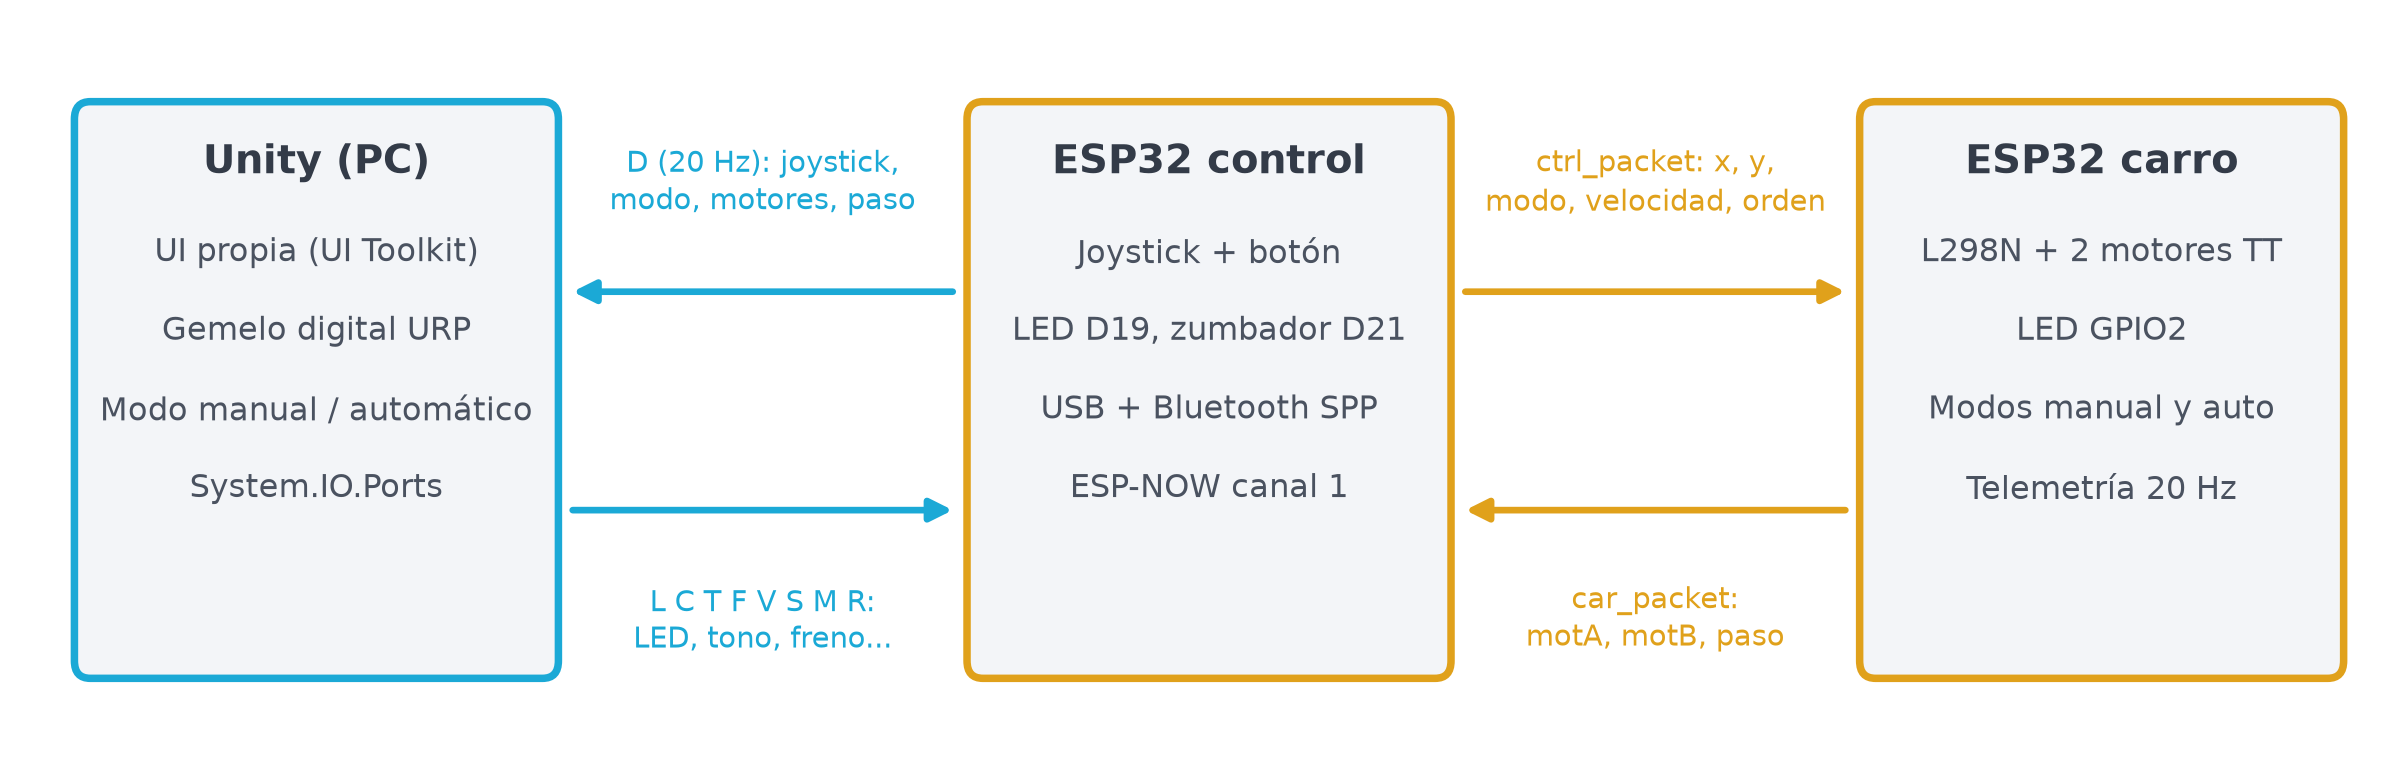
\includegraphics[width=\linewidth]{figs/arquitectura.png}
\caption{Arquitectura: Unity se comunica con el control por USB o Bluetooth SPP y el control con el carro por ESP-NOW.}
\label{fig:arq}
\end{figure}

\subsection{Coexistencia de ESP-NOW y Bluetooth}
El ESP32 clásico tiene una única radio de 2.4~GHz que se reparte por tiempo entre Wi-Fi y Bluetooth mediante coexistencia por software \cite{coexist}. ESP-NOW funciona sobre la capa Wi-Fi en modo estación sin conectarse a un punto de acceso \cite{espnow}, por lo que puede convivir con Bluetooth Clásico SPP. Ambas placas usan ESP32-WROOM (chip revisión~3, identificado por el arranque \texttt{ets Jul 29 2019}), que sí soporta Bluetooth Clásico; los modelos ESP32-S3 o C3 solo tienen BLE. Se fijó el canal 1 en ambos equipos. El firmware del control con Bluetooth y Wi-Fi ocupa 1\,621\,603 bytes, más que la partición por defecto de 1.2~MB, por lo que se usa la partición \emph{Huge APP} de 3~MB. El USB queda como alternativa con el mismo protocolo.

\subsection{Firmware del carro}
Se reescribió sin el sensor HC-SR04. Conserva la mezcla tipo tanque del modo manual, la pausa de 120~ms al invertir el giro, el impulso de arranque y la rutina automática de 25~s (espera, avanza, gira a la derecha, avanza, gira a la izquierda y retrocede). Se agregaron: un límite de velocidad de 0 a 100~\% aplicado al PWM, freno activo y vibración (pulsos alternos de 45~ms) por tiempo definido, el LED integrado (GPIO2) con cinco patrones, y el envío de telemetría al control cada 50~ms. La dirección del control se aprende del primer paquete recibido, de modo que el carro no necesita la MAC del control. El carro sigue aceptando el paquete anterior de 5~bytes.

\subsection{Firmware del control}
Lee el joystick con zona muerta, cambia de modo con el botón y envía cada 50~ms el paquete \texttt{ctrl\_packet} al carro. Lee líneas de texto por USB y por Bluetooth, las interpreta y reenvía las órdenes al carro con un identificador incremental para que cada orden se ejecute una sola vez. Si Unity deja de comunicarse por 3~s, el control vuelve al comportamiento original (LED indica el modo y velocidad al 100~\%), lo que mantiene el carro usable sin computador.

\section{Protocolo de comunicación}
Se eligió texto ASCII terminado en salto de línea a 115\,200 baudios por ser fácil de depurar con el Monitor Serie y de procesar en C\#. La Tabla~\ref{tab:proto} lista los mensajes.

\begin{table}[t]
\centering
\caption{Mensajes entre Unity y el control}
\label{tab:proto}
\begin{tabular}{@{}lll@{}}
\toprule
Sentido & Mensaje & Uso \\
\midrule
C$\rightarrow$U & \texttt{H,CarroRM,2.0} & saludo \\
C$\rightarrow$U & \texttt{D,x,y,m,e,a,b,p,s,v} & estado a 20 Hz \\
C$\rightarrow$U & \texttt{E,BTN,m} & botón pulsado \\
U$\rightarrow$C & \texttt{?}, \texttt{P} & saludo, mantener vivo \\
U$\rightarrow$C & \texttt{M,m} & modo manual/automático \\
U$\rightarrow$C & \texttt{L,p}, \texttt{C,p} & LED control / carro \\
U$\rightarrow$C & \texttt{T,f,ms} & tono del zumbador \\
U$\rightarrow$C & \texttt{F,ms}, \texttt{V,ms} & freno, vibración \\
U$\rightarrow$C & \texttt{S,0-100} & velocidad permitida \\
U$\rightarrow$C & \texttt{R} & reiniciar rutina \\
\bottomrule
\end{tabular}
\end{table}

En \texttt{D}, \texttt{x} e \texttt{y} son el joystick ($-1000$ a $1000$), \texttt{m} el modo, \texttt{e} si hay enlace con el carro, \texttt{a} y \texttt{b} el PWM real de cada lado ($-255$ a $255$), \texttt{p} el paso de la rutina, \texttt{s} el estado (freno, vibración) y \texttt{v} la velocidad permitida.

En Unity, la clase \texttt{SerialLink} abre el puerto en un hilo propio (los puertos Bluetooth pueden tardar varios segundos en abrir), lee bytes con un tiempo de espera de 40~ms y entrega líneas completas al hilo principal por una cola concurrente. La clase \texttt{Hub} hace el saludo, interpreta los mensajes, envía el mantenimiento cada 0.5~s y declara la conexión perdida si pasan 2.5~s sin datos. Para usar \texttt{System.IO.Ports} \cite{ports} se configuró el nivel de compatibilidad .NET Framework.

\section{Experiencia en Unity}
\subsection{Flujo}
La Fig.~\ref{fig:flujo} muestra el recorrido del usuario. Si la conexión se pierde en cualquier pantalla, la aplicación avisa y vuelve a la de conexión.

\begin{figure}[t]
\centering
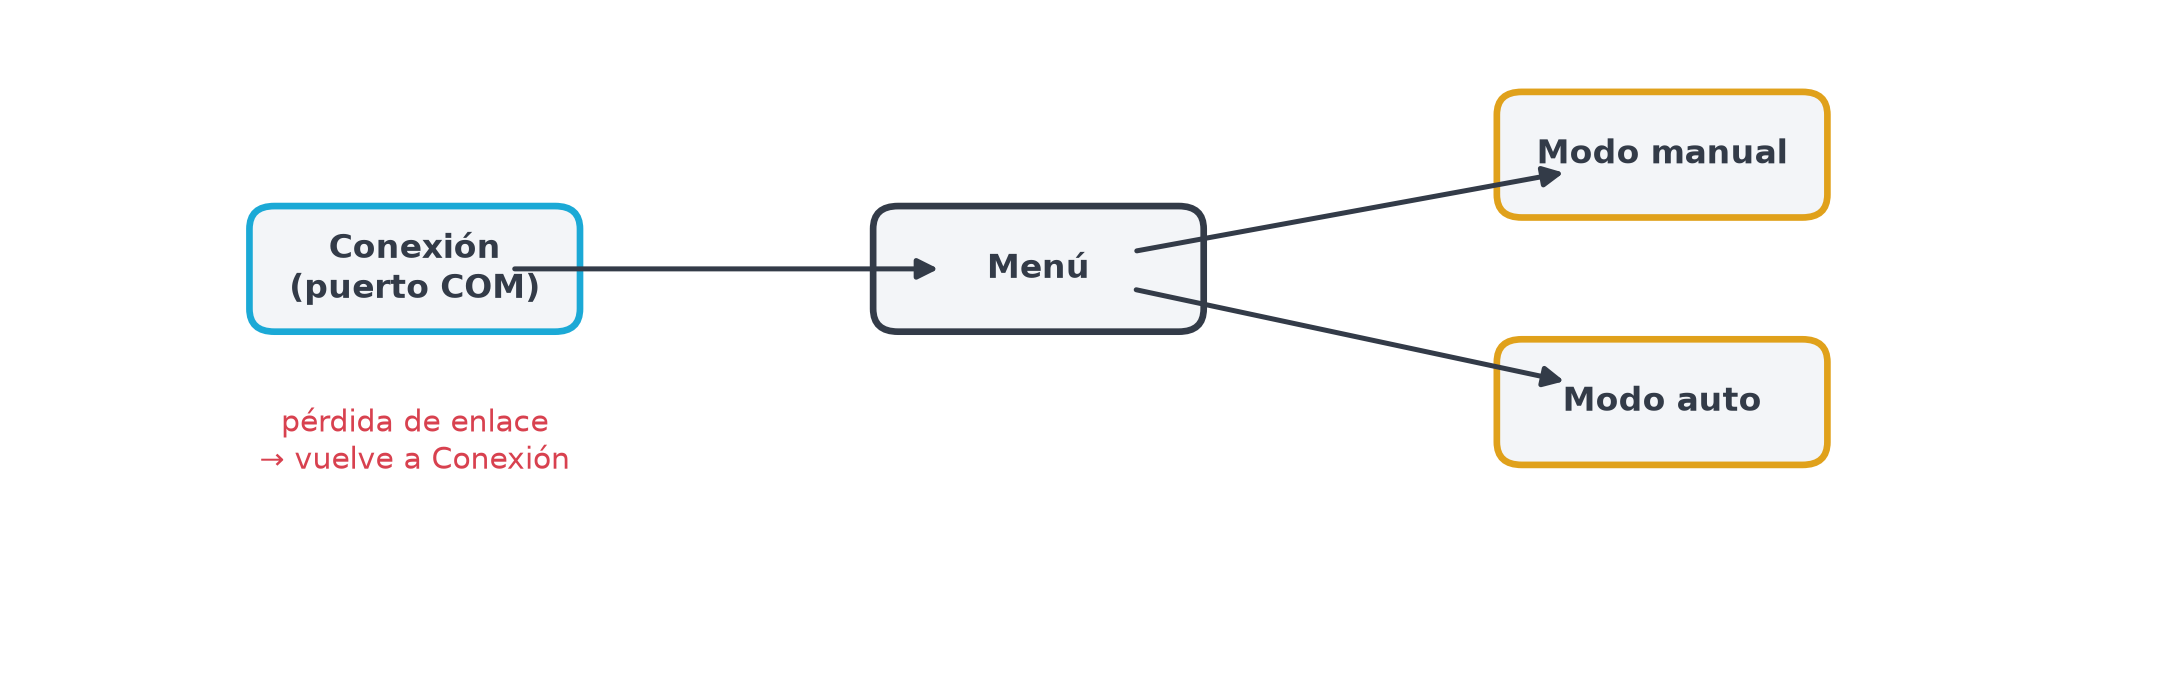
\includegraphics[width=\linewidth]{figs/flujo.png}
\caption{Flujo de pantallas de la aplicación.}
\label{fig:flujo}
\end{figure}

\subsection{Selección del puerto}
Como el producto es un ejecutable, el puerto se elige en la propia interfaz (Fig.~\ref{fig:con}). La lista se actualiza sola cada 2.5~s y clasifica cada puerto leyendo el registro de Windows (\texttt{HARDWARE\textbackslash DEVICEMAP\textbackslash SERIALCOMM}): los nombres \texttt{BthModem} son Bluetooth y los de controladores como Silabser o CH340 son USB. Los errores se explican en lenguaje claro: puerto ocupado por el Monitor Serie, puerto que corresponde al ESP32 del carro (se reconoce por su mensaje de arranque), dispositivo que no responde o conexión perdida. Un modo de demostración con teclado permite revisar la experiencia sin hardware. La interfaz se dejó deliberadamente mínima: cada pantalla muestra solo lo necesario para la tarea.

\begin{figure}[t]
\centering
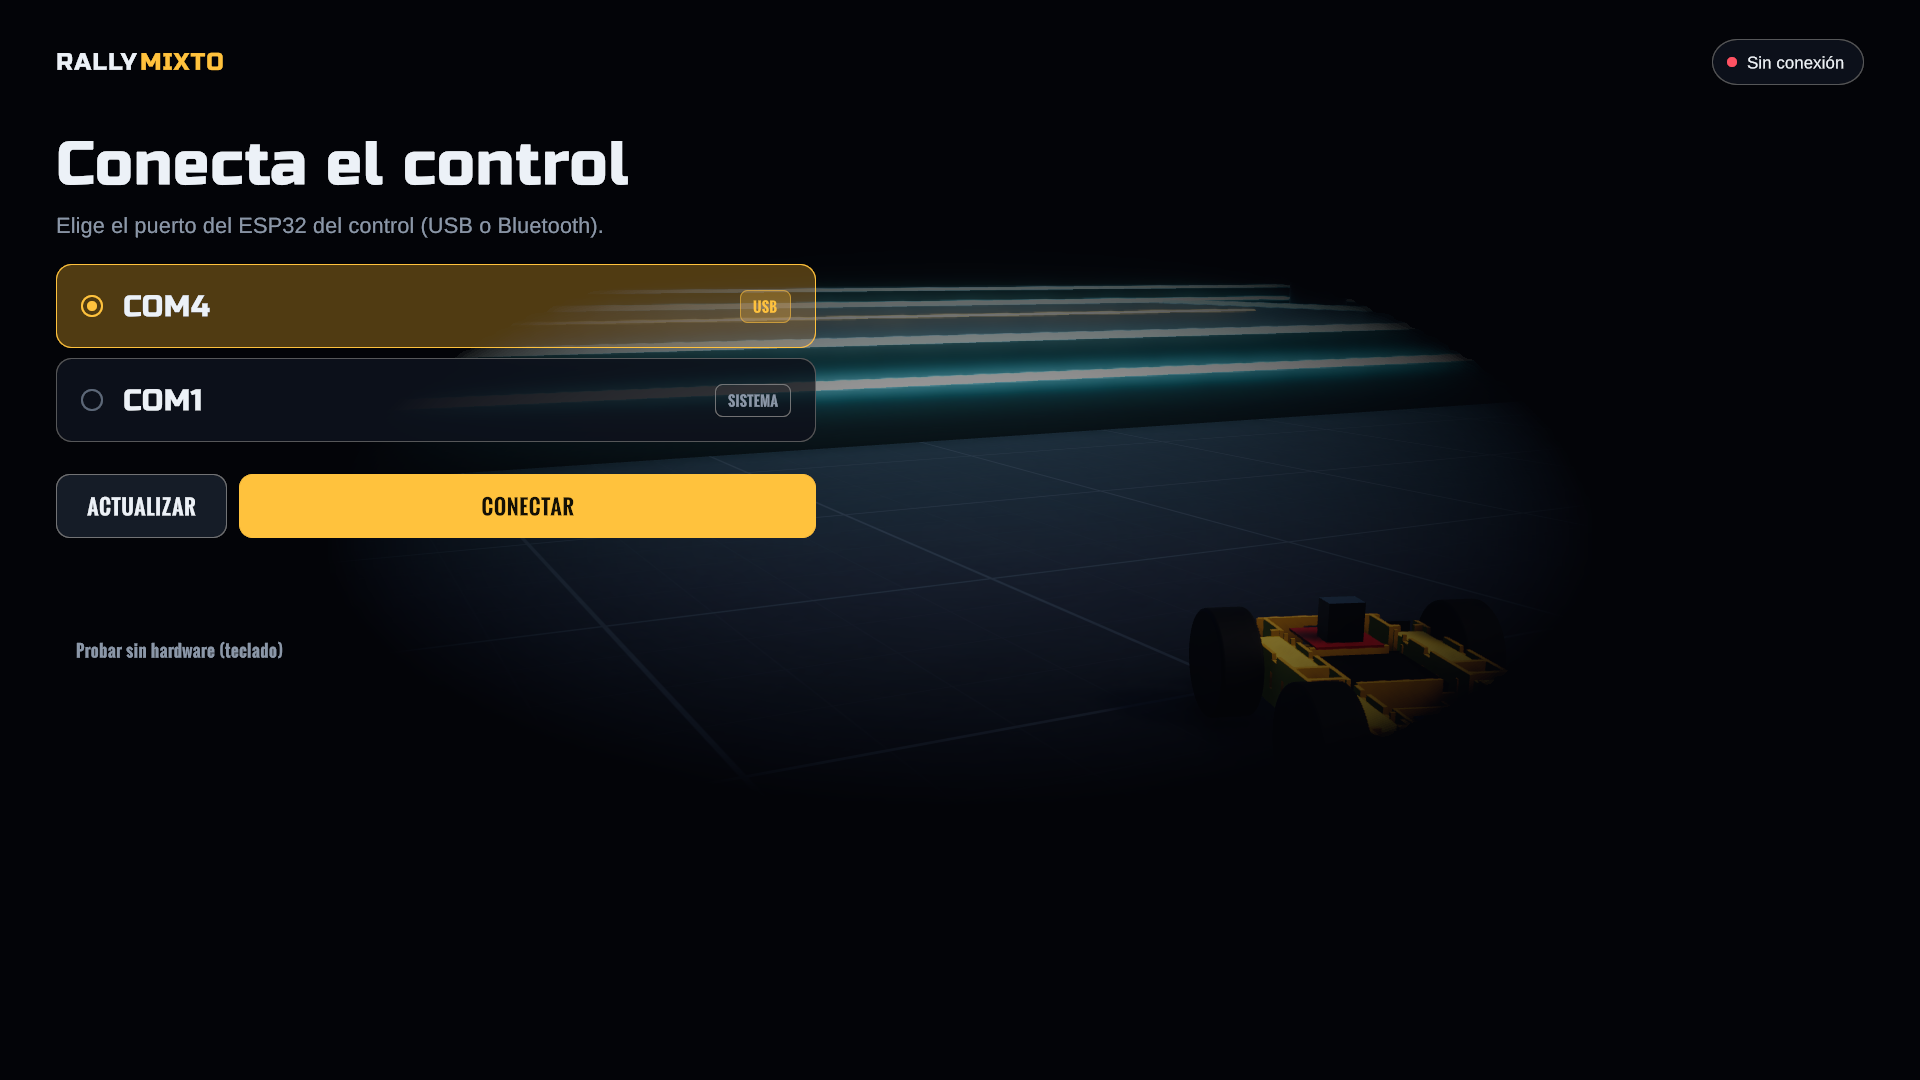
\includegraphics[width=\linewidth]{../capturas/02_conexion.png}
\caption{Pantalla de conexión con los puertos detectados.}
\label{fig:con}
\end{figure}

\subsection{Modo manual}
El joystick maneja el carro real y, al mismo tiempo, el gemelo digital en una pista con muros (Fig.~\ref{fig:man}). El gemelo se mueve con la telemetría del carro: la velocidad lineal es el promedio del PWM de ambos lados y la angular su diferencia, igual que la tracción diferencial del vehículo. Si el carro no tiene enlace, Unity aplica la misma mezcla del firmware sobre el joystick. La Tabla~\ref{tab:retro} resume la retroalimentación.

\begin{table}[t]
\centering
\caption{Eventos en Unity y retroalimentación al hardware}
\label{tab:retro}
\begin{tabular}{@{}lll@{}}
\toprule
Evento & Visual / sonora & Física (carro) \
\midrule
Entrar al menú & LED fijo & velocidad 0 \% \
Entrar a modo manual & LED fijo (control y carro) & velocidad 100 \% \
Choque con muro & LED rápido + 140 Hz & freno 400 ms \
Paso de la rutina & destello + 660 Hz & --- \
Fin de la rutina & LED fijo + melodía & --- \
\bottomrule
\end{tabular}
\end{table}

\begin{figure}[t]
\centering
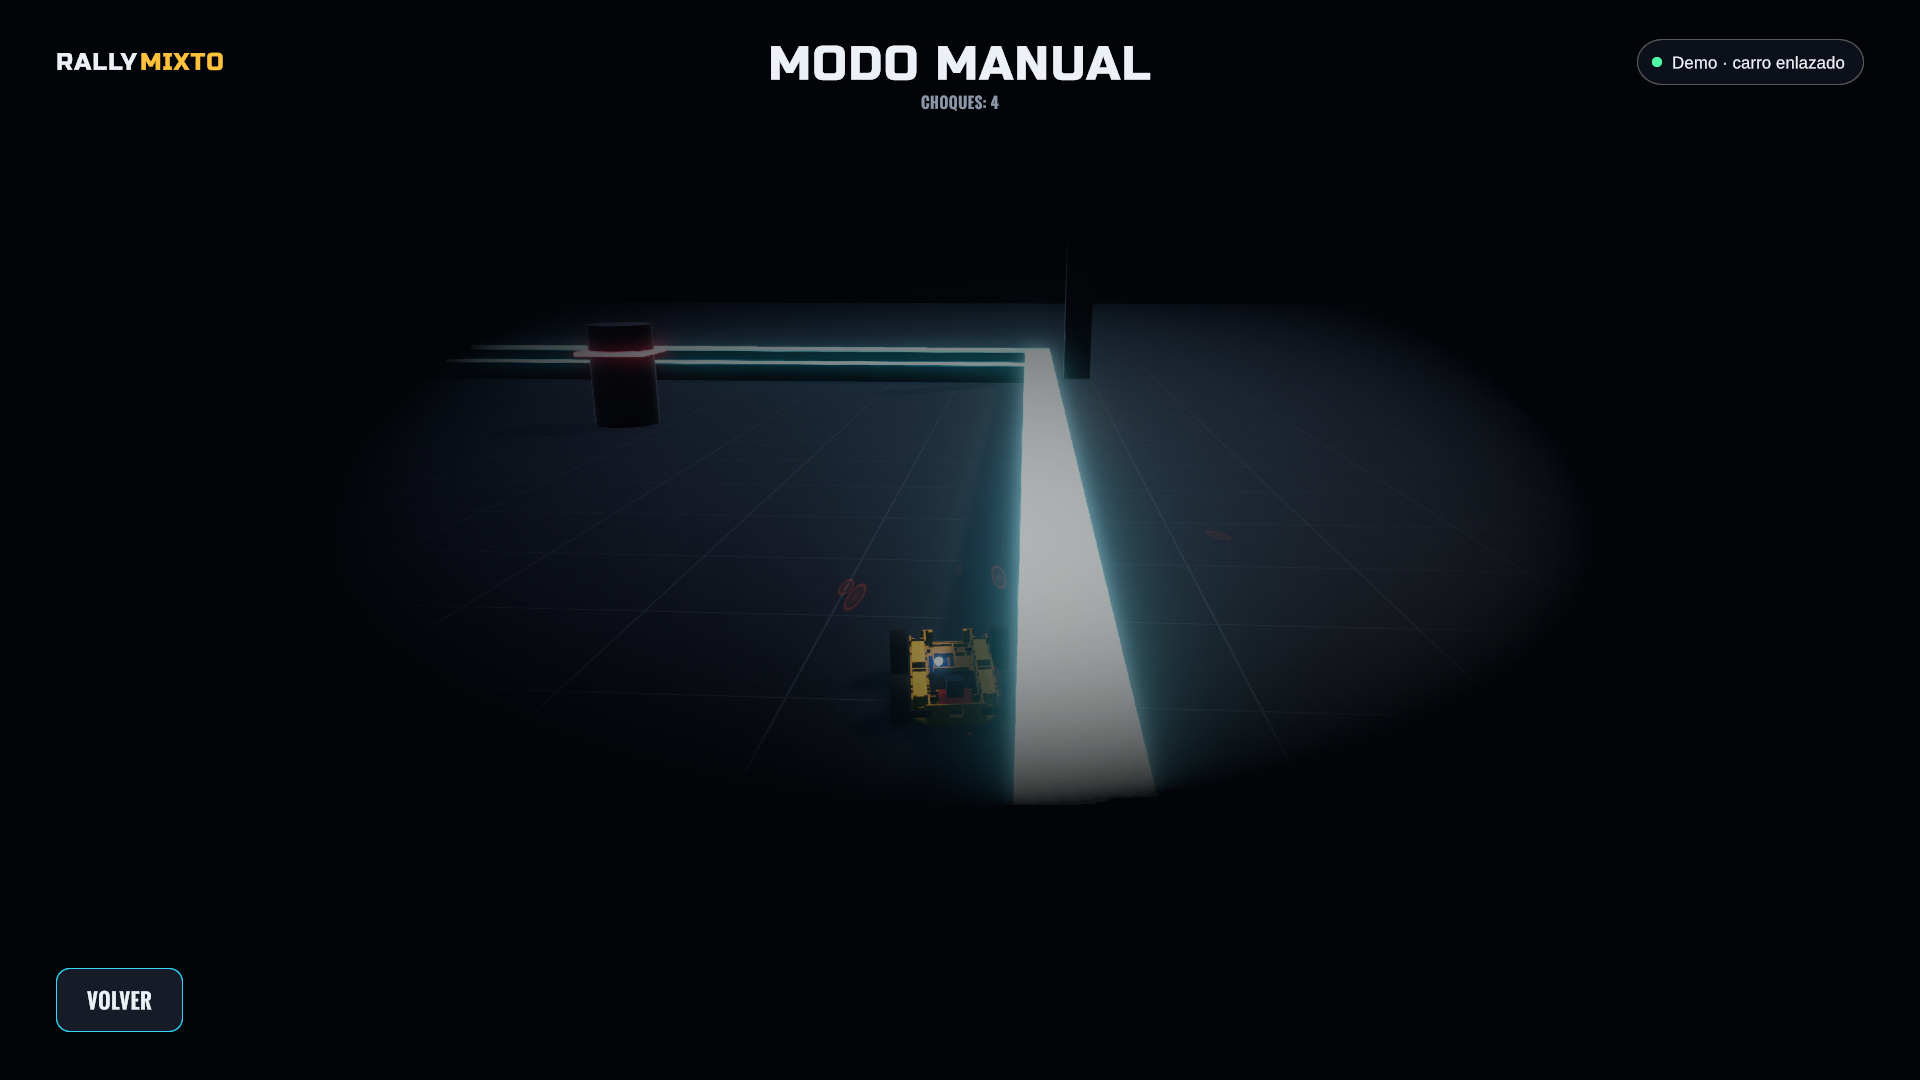
\includegraphics[width=\linewidth]{../capturas/04_manual.png}
\caption{Modo manual: el gemelo digital sigue al carro real.}
\label{fig:man}
\end{figure}

\subsection{Modo automático}
En el modo automático el carro ejecuta su rutina y Unity resalta el paso que reporta el carro, mientras el gemelo reproduce el movimiento (Fig.~\ref{fig:auto}). Cada cambio de paso produce un destello y un tono. Si no hay telemetría, el gemelo sigue la rutina por tiempo y la interfaz lo indica.

\begin{figure}[t]
\centering
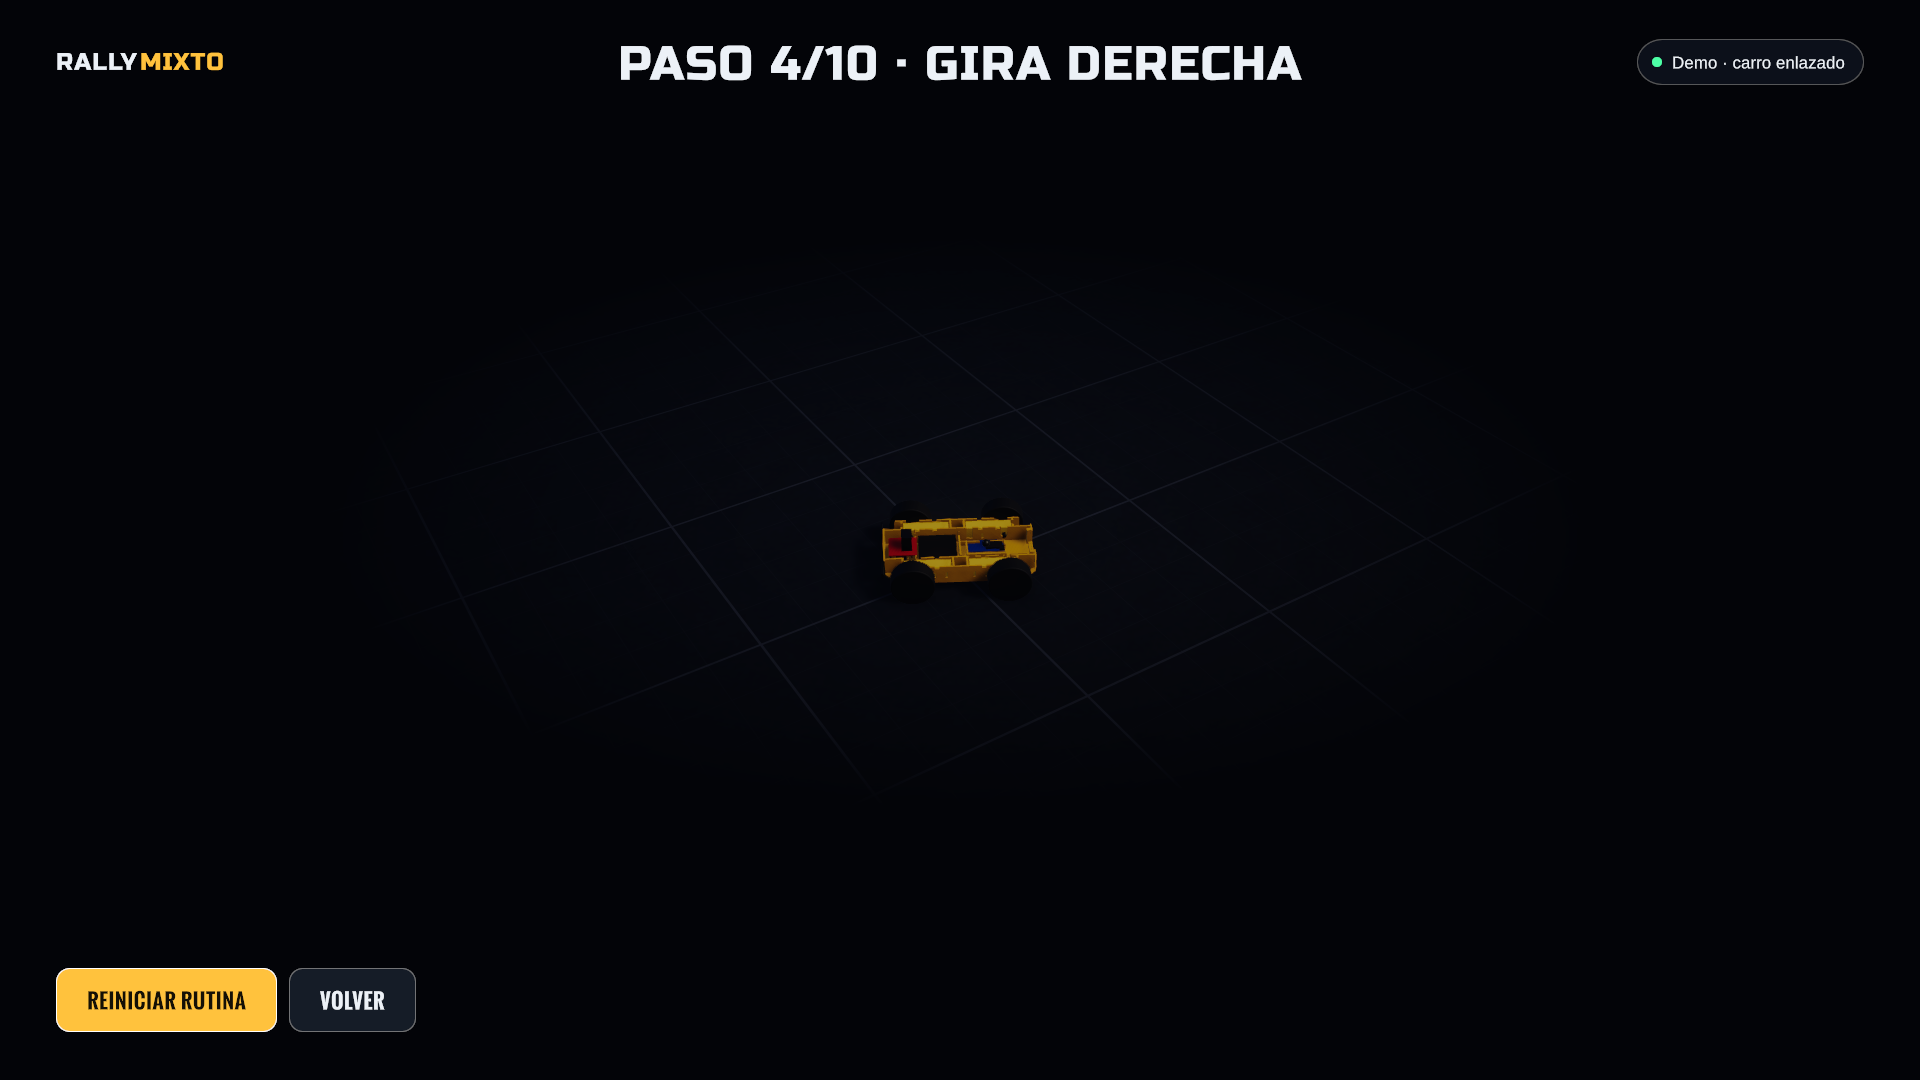
\includegraphics[width=\linewidth]{../capturas/09_automatico.png}
\caption{Modo automático: paso actual de la rutina.}
\label{fig:auto}
\end{figure}

\subsection{Diseño visual y de interacción}
No se usaron elementos de interfaz por defecto de Unity. La interfaz se construyó con UI Toolkit \cite{uitk} y un tema vacío y estilos propios en USS, con una composición mínima: título, lista o tarjetas y un botón principal por pantalla. El código de color separa los dominios: ámbar para lo físico y cian para lo digital, rojo para choques y violeta para sonido. Las tipografías son de licencia libre (Russo One, Oswald, Liberation Sans). Los botones tienen estados de foco, paso del ratón y pulsación, con sonidos sintetizados en tiempo de ejecución. La escena usa URP con luces puntuales, neón emisivo, sonda de reflejos, \emph{bloom}, mapeo de tonos ACES y viñeta. El modelo 3D del carro se exportó desde el diseño CAD del chasis en Blender, sin el sensor y con el L298N.

\section{Pruebas y resultados}
\begin{table}[t]
\centering
\caption{Verificaciones realizadas}
\label{tab:pruebas}
\begin{tabular}{@{}p{4.4cm}p{3.2cm}@{}}
\toprule
Prueba & Resultado \\
\midrule
Compilación firmware carro (core 3.3.12) & 898\,583 B (68 \%) \\
Compilación firmware control (Huge APP) & 1\,621\,603 B (51 \%) \\
Build Windows (Unity 6000.3.8f1) & 95 MB, 37 MB comprimido \\
Detección de puertos en el PC & COM4 USB, COM1 sistema \\
Arranque del carro por COM4 & MAC EC:C9:FF:FE:85:C8 \\
Recorrido completo en modo demo & sin errores \\
Rendimiento 1920$\times$1080 & 72 fps (sincronía vertical) \\
Datos recibidos en Unity (demo) & 18 a 20 Hz \\
Latencia joystick $\rightarrow$ gemelo & \pend{medir} \\
Latencia orden $\rightarrow$ carro & \pend{medir} \\
Pérdida de paquetes con BT activo & \pend{medir} \\
\bottomrule
\end{tabular}
\end{table}

La Tabla~\ref{tab:pruebas} resume lo verificado. La carga del nuevo firmware al carro desde el PC falló porque la placa no entra sola en modo de descarga (\emph{Wrong boot mode}); se resuelve manteniendo presionado BOOT al iniciar la carga. Las mediciones con el hardware completo quedan pendientes. Para la latencia se propone filmar a 240~fps el joystick y la pantalla, y contar cuadros entre el movimiento y la respuesta; para la pérdida, contar paquetes recibidos por el carro durante 60~s con y sin Bluetooth conectado.

\section{Conclusiones}
El ESP32 clásico puede mantener ESP-NOW con el carro y Bluetooth Clásico con el computador al mismo tiempo, siempre que se use una partición de memoria mayor. Centralizar la comunicación en el control evitó modificar el enlace del carro y permitió que Unity lea entradas y telemetría y responda con retroalimentación visual, sonora y física. La interfaz propia, la selección del puerto en pantalla y los mensajes de error claros hacen que el ejecutable pueda usarse sin conocer el código.

\begin{thebibliography}{1}
\bibitem{espnow} Espressif Systems, ``ESP-NOW,'' \emph{ESP-IDF Programming Guide}, v5.4. [En línea]. Disponible: \url{https://docs.espressif.com/projects/esp-idf/en/v5.4/esp32/api-reference/network/esp_now.html}
\bibitem{coexist} Espressif Systems, ``RF Coexistence,'' \emph{ESP-IDF Programming Guide}. [En línea]. Disponible: \url{https://docs.espressif.com/projects/esp-idf/en/latest/esp32/api-guides/coexist.html}
\bibitem{uitk} Unity Technologies, ``UI Toolkit,'' \emph{Unity Manual}, 2026. [En línea]. Disponible: \url{https://docs.unity3d.com/Manual/UIElements.html}
\bibitem{ports} Microsoft, ``SerialPort Class,'' \emph{.NET Framework Documentation}. [En línea]. Disponible: \url{https://learn.microsoft.com/dotnet/api/system.io.ports.serialport}
\end{thebibliography}

\end{document}
